%#################### 9.1 ####################
\subsection{\hll{LaTeX Coffee Stains}}
 
\begin{tabular}{c | c}
\begin{minipage}[m]{0.4\textwidth}
\enum{\cofeAm{1}{0.6}{0}{0.cm}{6.5cm} 

\cofeCm{0.9}{0.5}{180}{-7.cm}{11cm}

Download \fbox{coffee4.sty} and put in the same directory

\cofeDm{0.2}{0.2}{90}{0.5cm}{2.5cm}
\cofeBm{0.5}{0.5}{0}{-3.cm}{10cm}

 }{\href{https://www.overleaf.com/latex/examples/latex-coffee-stains/qsjjwwsrmwnc}{\thesubsection}}

\end{minipage}
&
\begin{minipage}[m]{0.55\textwidth}
\renewcommand\textminus{\mbox{-}}%<<<<<<<<<<<

\begin{lstlisting}[numberstyle=\zebra{orange!15}{red!15},numbers=left,basicstyle=\ttfamily\footnotesize]
\documentclass{article}
\usepackage{tikz}
\usetikzlibrary{arrows,shapes}
\usepackage{coffee4}
\cofeAm{1}{0.6}{0}{0.cm}{6cm} 
\cofeCm{0.9}{0.5}{180}{-7.cm}{11cm}
\cofeDm{0.4}{0.2}{90}{1.0cm}{3.0cm}
\cofeBm{0.5}{0.5}{0}{-3.cm}{10cm}
%\cofeAm{alpha}{scale}{angle}{xoff}{yoff} <-- usage
\end{document}
\end{lstlisting}
\end{minipage}
\end{tabular}
 
%#################### 9.2 ####################
\subsection{\hll{Sticky notes}}
 
\begin{tabular}{c | c}
\begin{minipage}[m]{0.4\textwidth}
\enum{ \href{https://tex.stackexchange.com/questions/26846/how-to-scale-a-tikzpicture-including-texts}{\img{1}{9.3}}}{\thesubsection}

\end{minipage}
&
\begin{minipage}[m]{0.55\textwidth}
\renewcommand\textminus{\mbox{-}}%<<<<<<<<<<<
\begin{lstlisting}[numberstyle=\zebra{orange!15}{red!15},numbers=left,basicstyle=\ttfamily\scriptsize]
\documentclass{article}
\usepackage{xparse}
\usepackage{fancypar}
\usetikzlibrary{calc,shadows}
\NewDocumentCommand\StickyNoteP{O{6cm}mO{6cm}}{%
\begin{tikzpicture}
\node[
drop shadow={shadow xshift=3pt,},
inner xsep=0pt,
xslant=-0.1,yslant=0.1,
inner ysep=0pt,
text depth=\the\dimexpr#1+2.5ex\relax
] {\parbox[t][#1][c]{#3}{#2}};
\end{tikzpicture}}

\begin{document}
\StickyNoteP[2.5cm]{%
\NotebookPar[spiral=false]{
\LARGE first\\  second }}[6.5cm]
\end{document}
\end{lstlisting}
\end{minipage}
\end{tabular}
 
\clearpage
%#################### 9.3 ####################
\subsection{\hll{\fadingtext[scale=1, font=\bfseries]{path picture shading=rainbow}{Rainbow text}}}
 
\begin{tabular}{c | c}
\begin{minipage}[m]{0.4\textwidth}
\enum{
\fadingtext[scale=2, font=\bfseries]{upper left=red, upper right=green, lower left=blue,lower right=yellow}{\LaTeX} 
\fadingtext[scale=2, font=\bfseries]{path picture shading=rainbow}{\LaTeX} \\

\noindent\fadingtext[scale=0.7, font=\bfseries]{path picture shading=rainbow}{\parbox[b]{1.5\linewidth}{\strut\lipsum[1]}}

 }{\href{https://tex.stackexchange.com/questions/344260/rainbow-colored-one-letter-with-tikz-and-xcolor}{9.3}}

\end{minipage}
&
\begin{minipage}[m]{0.55\textwidth}
\renewcommand\textminus{\mbox{-}}%<<<<<<<<<<<
\begin{lstlisting}[numberstyle=\zebra{orange!15}{red!15},numbers=left,basicstyle=\ttfamily\scriptsize]
  \documentclass{article} 
  \usepackage{tikz}
  \usetikzlibrary{fadings, shadings}
  \newcounter{fadcnt}\setcounter{fadcnt}{0}
  \newcommand\fadingtext[3][]{%
  \stepcounter{fadcnt}
    \begin{tikzfadingfrompicture}[name=fading letter\thefadcnt]
      \node[text=transparent!0,inner xsep=0pt,outer xsep=0pt,#1] {#3};
    \end{tikzfadingfrompicture}%
    \begin{tikzpicture}[baseline=(textnode.base)]
      \node[inner sep=0pt,outer sep=0pt,#1](textnode){\phantom{#3}}; 
      \shade[path fading=fading letter\thefadcnt,#2,fit fading=false]
      (textnode.south west) rectangle (textnode.north east);% 
    \end{tikzpicture}% 
  }
  \usetikzlibrary{calc}
  \newbox\shbox
  \tikzset{%
    path picture shading/.style={%
    path picture={%
  %
  \pgfpointdiff{\pgfpointanchor{path picture bounding box}{south west}}%
    {\pgfpointanchor{path picture bounding box}{north east}}%
  \pgfgetlastxy\pathwidth\pathheight%
  \pgfinterruptpicture%
     \global\setbox\shbox=\hbox{\pgfuseshading{#1}}%
   \endpgfinterruptpicture%
  \pgftransformshift{\pgfpointanchor{path picture bounding box}{center}}%
  \pgftransformxscale{\pathwidth/(\wd\shbox)}%
  \pgftransformyscale{\pathheight/(\ht\shbox)}% \dp will (should) be 0pt
  \pgftext{\box\shbox}%
  %
      }
    }
  }
  \pgfdeclarehorizontalshading{rainbow}{10bp}{color(0bp)=(violet);
              color(1.6667bp)=(blue);
              color(3.3333bp)=(cyan);
              color(5bp)=(green);
              color(6.6667bp)=(yellow);
              color(8.3333bp)=(orange);
              color(10bp)=(red)}
  \begin{document} 
   \fadingtext[scale=10, font=\bfseries]{upper left=red, upper right=green, lower left=blue,lower right=yellow}{\LaTeX}

  \fadingtext[scale=10, font=\bfseries]{path picture shading=rainbow}{\LaTeX}

  \noindent\fadingtext[scale=0.7, font=\bfseries]{path picture shading=rainbow}{\parbox[b]{1.5\linewidth}{\strut\lipsum[1]}}
  \end{document}
\end{lstlisting}
\end{minipage}
\end{tabular}
 
 

%#################### 9.4 ####################
\subsection{\hll{Single Watermark}}
 
\begin{tabular}{c | c}
\begin{minipage}[m]{0.4\textwidth}
\enum{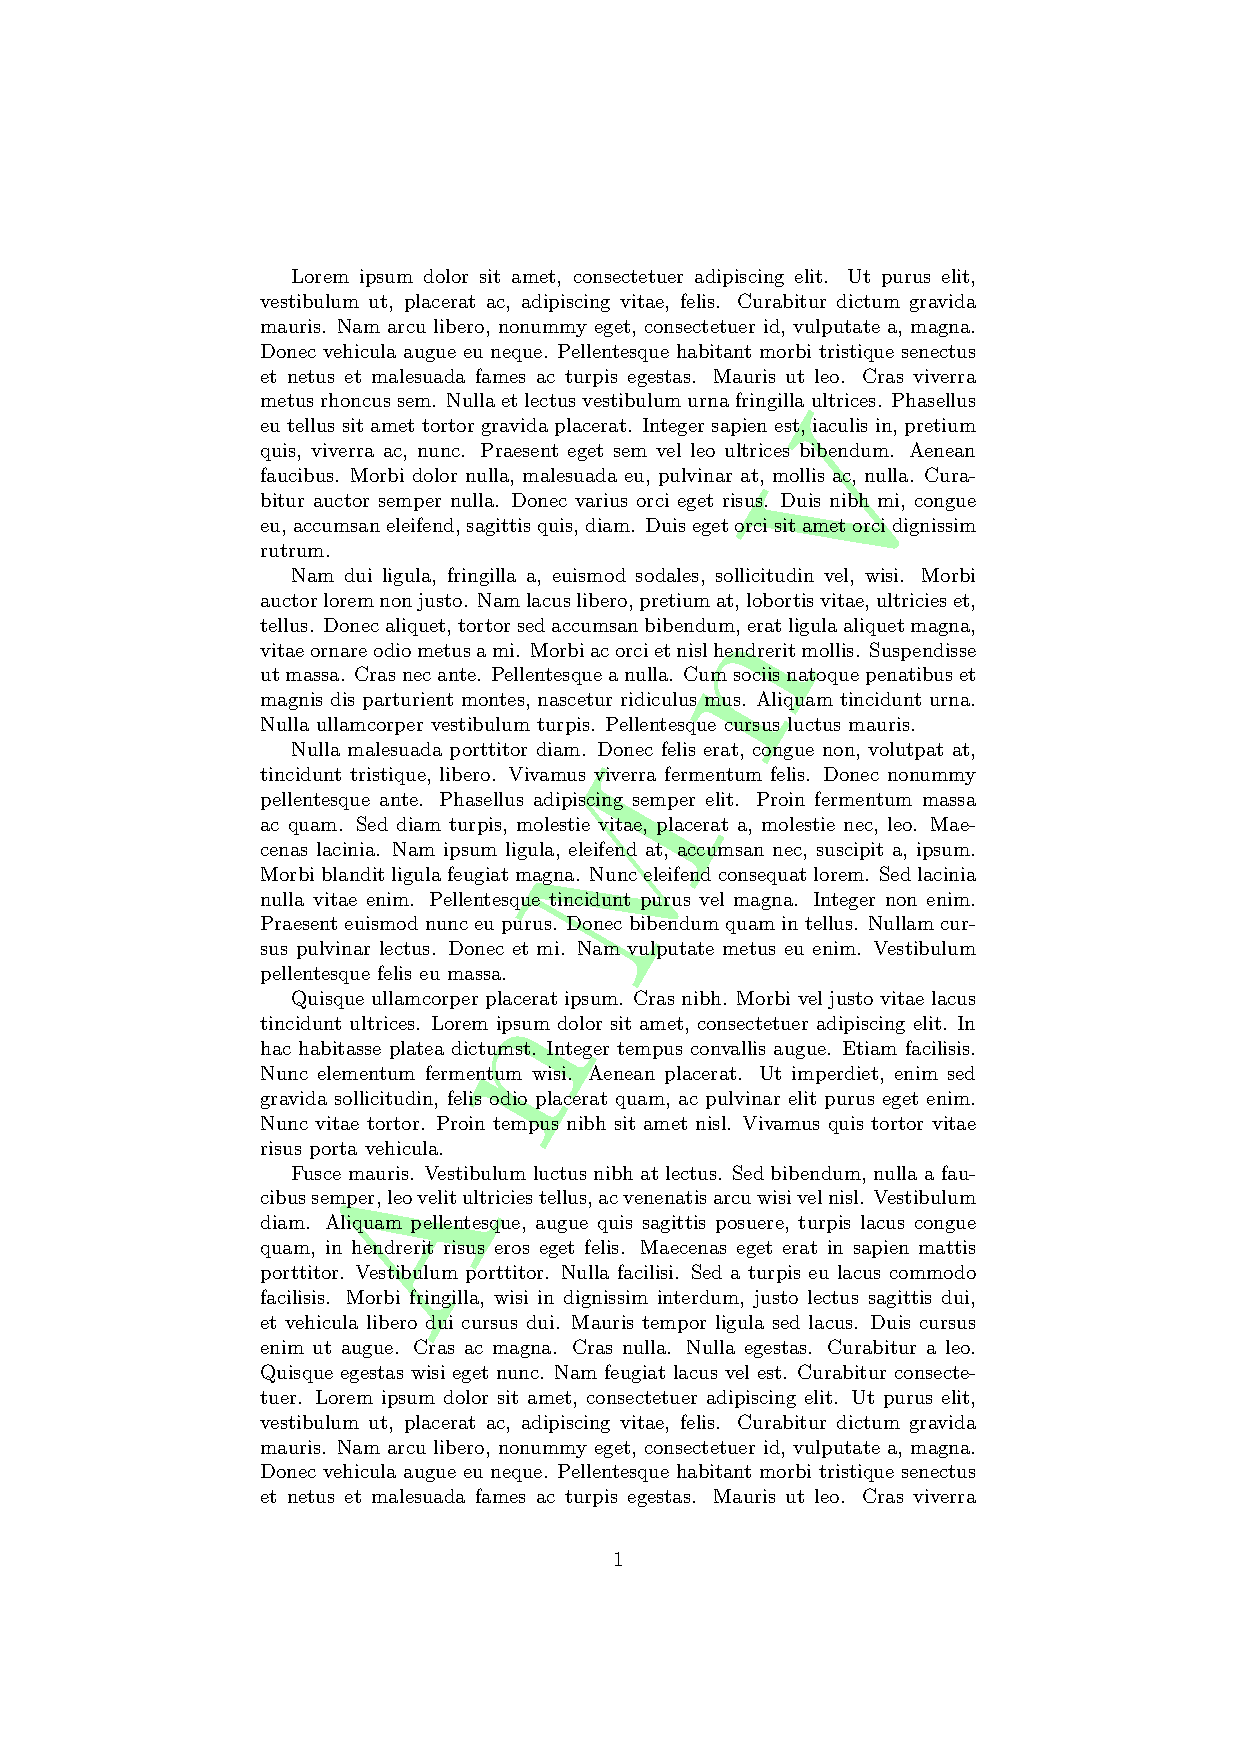
\includegraphics[width=0.9\linewidth]{C:/Users/user/Desktop/eBook/images/9.4/9.4.pdf}}{\thesubsection}

\end{minipage}
&
\begin{minipage}[m]{0.55\textwidth}
\renewcommand\textminus{\mbox{-}}%<<<<<<<<<<<
\begin{lstlisting}[numberstyle=\zebra{orange!15}{red!15},numbers=left,basicstyle=\ttfamily\scriptsize]
\documentclass[a4paper]{article}
\usepackage[T1]{fontenc}
\usepackage[utf8]{inputenc}
\usepackage[pages=some]{background}% change "some" to "all" to see WM on all pages 
\usepackage{lipsum}
\backgroundsetup{color=green, opacity=0.3, scale=10, contents={A n M n V}}

\begin{document}
\lipsum[1-5] 
\BgThispage
\lipsum[1-5]
\end{document}
\end{lstlisting}
\end{minipage}
\end{tabular}
 
%#################### 9.5 #################### 
\subsection{\hll{Full page of Watermarks}}
 
\begin{tabular}{c | c}
\begin{minipage}[m]{0.4\textwidth}
\enum{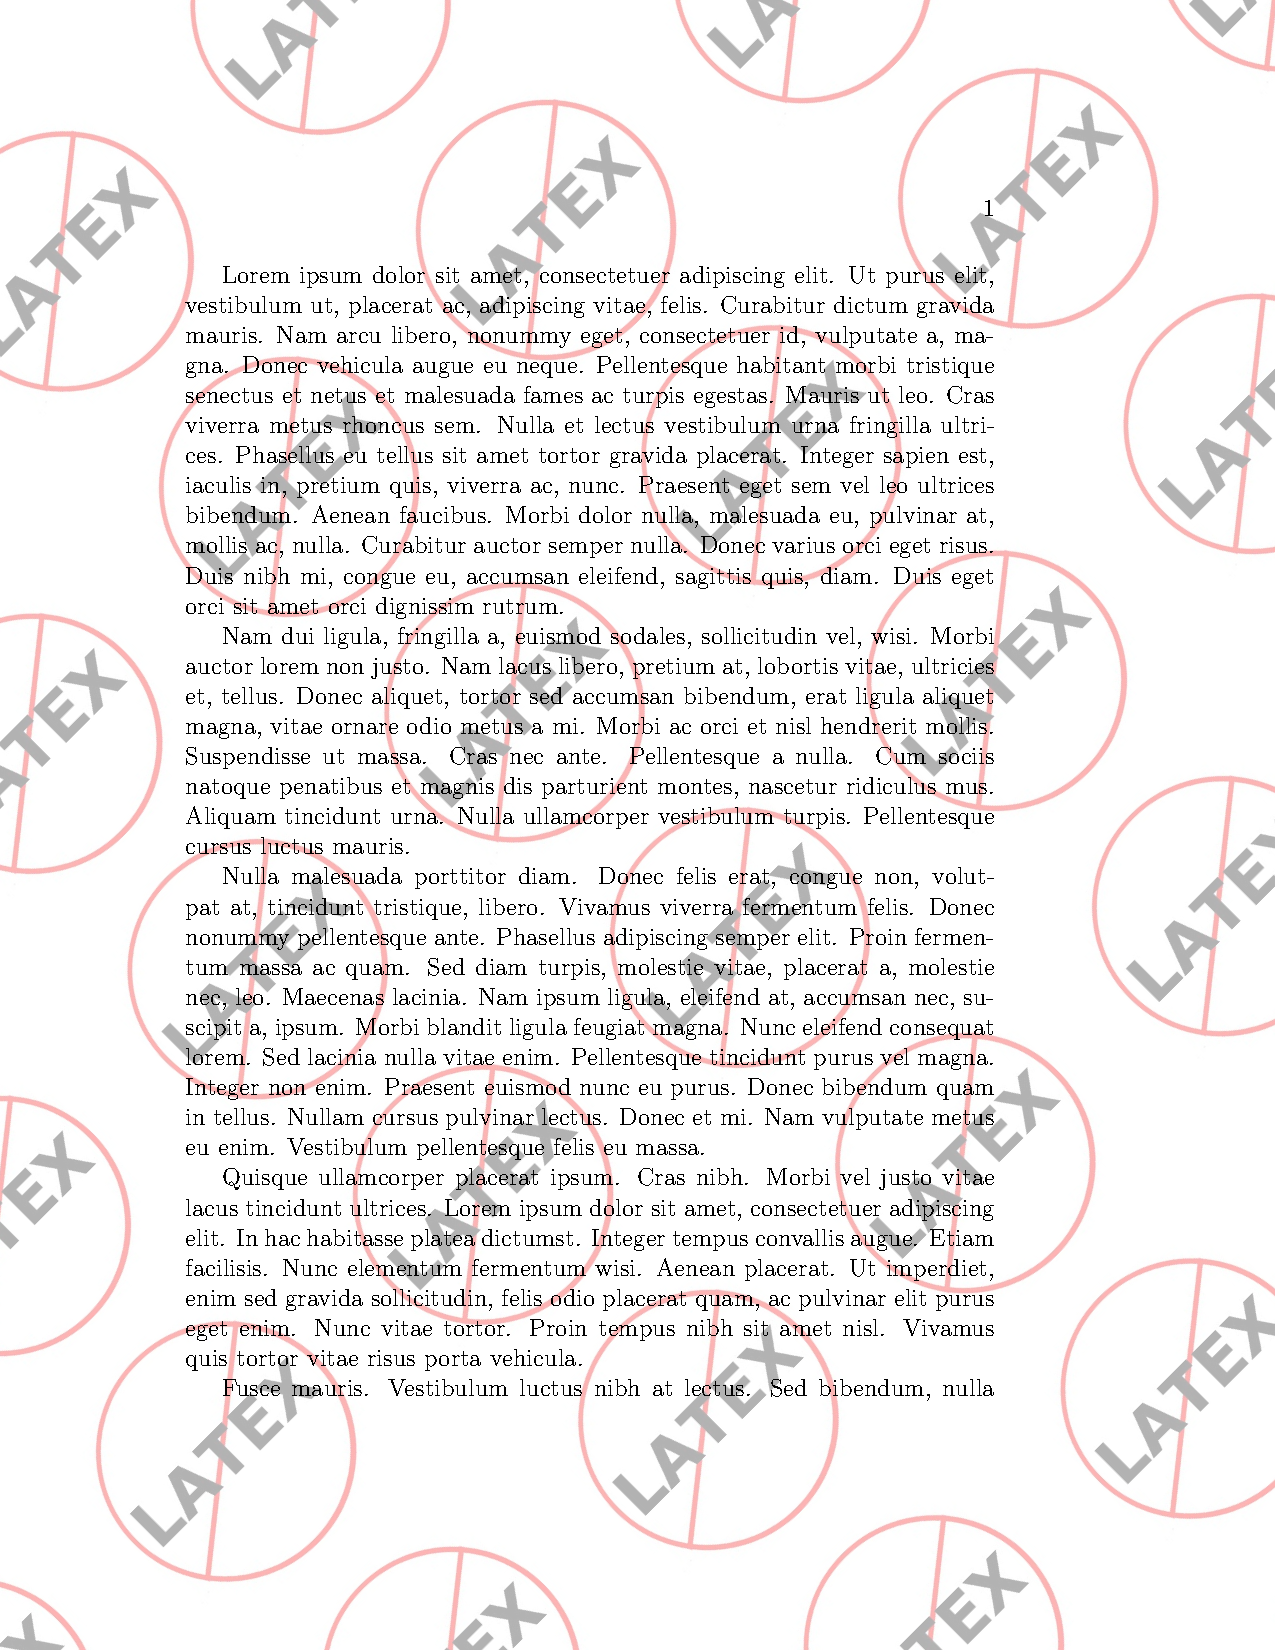
\includegraphics[width=0.9\linewidth]{C:/Users/user/Desktop/eBook/images/9.5/9.5.pdf}}{\thesubsection}

\end{minipage}
&
\begin{minipage}[m]{0.55\textwidth}
\renewcommand\textminus{\mbox{-}}%<<<<<<<<<<<
\begin{lstlisting}[numberstyle=\zebra{orange!15}{red!15},numbers=left,basicstyle=\ttfamily\scriptsize]
\documentclass[12pt]{book}
\usepackage{graphicx}
\usepackage[pages=some]{background}
\usepackage{lipsum}
\newcommand\DupImage{%
     
\includegraphics[width=5cm]{logo.jpeg}\hfill%  YOUR IMAGE
     
\includegraphics[width=5cm]{logo.jpeg}\hfill%  YOUR IMAGE
     
\includegraphics[width=5cm]{logo.jpeg}\hfill%  YOUR IMAGE
     
\includegraphics[width=5cm]{logo.jpeg}\hfill%  YOUR IMAGE
     
\includegraphics[width=5cm]{logo.jpeg}\hfill%  YOUR IMAGE
     
\includegraphics[width=5cm]{logo.jpeg}\hfill%  YOUR IMAGE
     
\includegraphics[width=5cm]{logo.jpeg}\hfill}
\newlength{\drop}
\backgroundsetup{  scale=1, angle=45, opacity=.3, 
  contents={%
     \begin{minipage}{1.5\paperheight}
     \DupImage\\[2ex]
     \DupImage\\[2ex]
     \DupImage\\[2ex]
     \DupImage\\[2ex]
     \DupImage\\[2ex]
     \DupImage\\[2ex]
     \DupImage\\[2ex]
     \DupImage\\[2ex]
     \DupImage\\[2ex]
     \DupImage  \end{minipage}   }  }

\begin{document}
\drop=0.1\textheight \BgThispage \lipsum[1-8]
\end{document}
\end{lstlisting}
\end{minipage}
\end{tabular}
 

%#################### 9.6 ####################
\subsection{\hll{Generating QR code}}
 
\begin{tabular}{c | c}
\begin{minipage}[m]{0.4\textwidth}
\enum{
\includegraphics[width=0.9\linewidth]{C:/Users/user/Desktop/eBook/images/9.6/9.6.pdf}}{\thesubsection}
\end{minipage}
&
\begin{minipage}[m]{0.55\textwidth}
\renewcommand\textminus{\mbox{-}}%<<<<<<<<<<<
\begin{lstlisting}[numberstyle=\zebra{orange!15}{red!15},numbers=left,basicstyle=\ttfamily\scriptsize]
\documentclass{article} 
\usepackage{qrcode} 

\begin{document}
\qrcode[height=0.5in]{https://github.com/AnMnv/eBook}
\textcolor{blue}{\qrcode[height=0.5in]{https://github.com/AnMnv/eBook}}
\textcolor{green}{\qrcode[height=0.5in]{https://github.com/AnMnv/eBook}} 
\end{document}
\end{lstlisting}
\end{minipage}
\end{tabular}
 





\newpage
%#################### 9.7 ####################https://tex.stackexchange.com/questions/560627/how-do-make-gradient-colored-qr-code-in-latex#655712
\subsection{\hll{Gradient QR code}}
 
\begin{tabular}{c | c}
\begin{minipage}[m]{0.4\textwidth}
\enum{
\includegraphics[width=0.9\linewidth]{C:/Users/user/Desktop/eBook/images/9.7/9.7.pdf}}{\thesubsection}
\end{minipage}
&
\begin{minipage}[m]{0.55\textwidth}
\renewcommand\textminus{\mbox{-}}%<<<<<<<<<<<
\begin{lstlisting}[numberstyle=\zebra{orange!15}{red!15},numbers=left,basicstyle=\ttfamily\scriptsize]
\documentclass{article} 
\usepackage{qrcode}[]
\usepackage{tikz}
\usetikzlibrary{fadings, shadings}
\newcounter{fadcnt}\setcounter{fadcnt}{0}
\newcommand\fadingtext[3][]{%
\stepcounter{fadcnt}
  \begin{tikzfadingfrompicture}[name=fading letter\thefadcnt]
    \node[text=transparent!0,inner xsep=0pt,outer xsep=0pt,#1] {#3};
  \end{tikzfadingfrompicture}%
  \begin{tikzpicture}[baseline=(textnode.base)]
    \node[inner sep=0pt,outer sep=0pt,#1](textnode){\phantom{#3}}; 
    \shade[path fading=fading letter\thefadcnt,#2,fit fading=false]
    (textnode.south west) rectangle (textnode.north east);% 
  \end{tikzpicture}}
\usetikzlibrary{calc}
\newbox\shbox
\tikzset{%
  path picture shading/.style={%
  path picture={%
\pgfpointdiff{\pgfpointanchor{path picture bounding box}{south west}}%
  {\pgfpointanchor{path picture bounding box}{north east}}%
\pgfgetlastxy\pathwidth\pathheight%
\pgfinterruptpicture%
   \global\setbox\shbox=\hbox{\pgfuseshading{#1}}%
 \endpgfinterruptpicture%
\pgftransformshift{\pgfpointanchor{path picture bounding box}{center}}%
\pgftransformxscale{\pathwidth/(\wd\shbox)}%
\pgftransformyscale{\pathheight/(\ht\shbox)}% \dp will (should) be 0pt
\pgftext{\box\shbox}%
    }  }  }
\pgfdeclarehorizontalshading{rainbow}{10bp}{color(0bp)=(violet);
            color(1.6667bp)=(blue);
            color(3.3333bp)=(cyan);
            color(5bp)=(green);
            color(6.6667bp)=(yellow);
            color(8.3333bp)=(orange);
            color(10bp)=(red)}
\pgfdeclareverticalshading{rainbow_vertical}{10bp}{color(0bp)=(violet);
            color(1.6667bp)=(blue);
            color(3.3333bp)=(cyan);
            color(5bp)=(green);
            color(6.6667bp)=(yellow);
            color(8.3333bp)=(orange);
            color(10bp)=(red)}

\begin{document}
\fadingtext[scale=0.5]{upper left=red, upper right=green, lower left=blue,lower right=yellow}{\qrcode[height=5cm]{https://github.com/AnMnv/eBook}}
\fadingtext[scale=0.5]{path picture shading=rainbow}{\qrcode[height=5cm]{https://github.com/AnMnv/eBook}}
\fadingtext[scale=0.5]{path picture shading=rainbow_vertical}{\qrcode[height=5cm]{https://github.com/AnMnv/eBook}}
\end{document}
\end{lstlisting}
\end{minipage}
\end{tabular}
 

%#################### 9.8 ####################LobLib documentation on \href{https://github.com/AnMnv/eBook}{GitHub} in \mybox[black]{LobLib-package} folder.\\ Origins of the package \href{https://github.com/bryce-evans/LobLib}{https://github.com/bryce-evans/LobLib}\\ However, to print lobsters put \mybox[red]{objects} folder and \mybox[red]{loblib.sty} from  the \mybox[black]{LobLib-package} folder into the same directory with your \mybox[brown]{.tex} file.
\subsection{\hll{Lobsrets}}
\begin{tabular}{c | c}
\begin{minipage}[m]{0.4\textwidth}
\enum{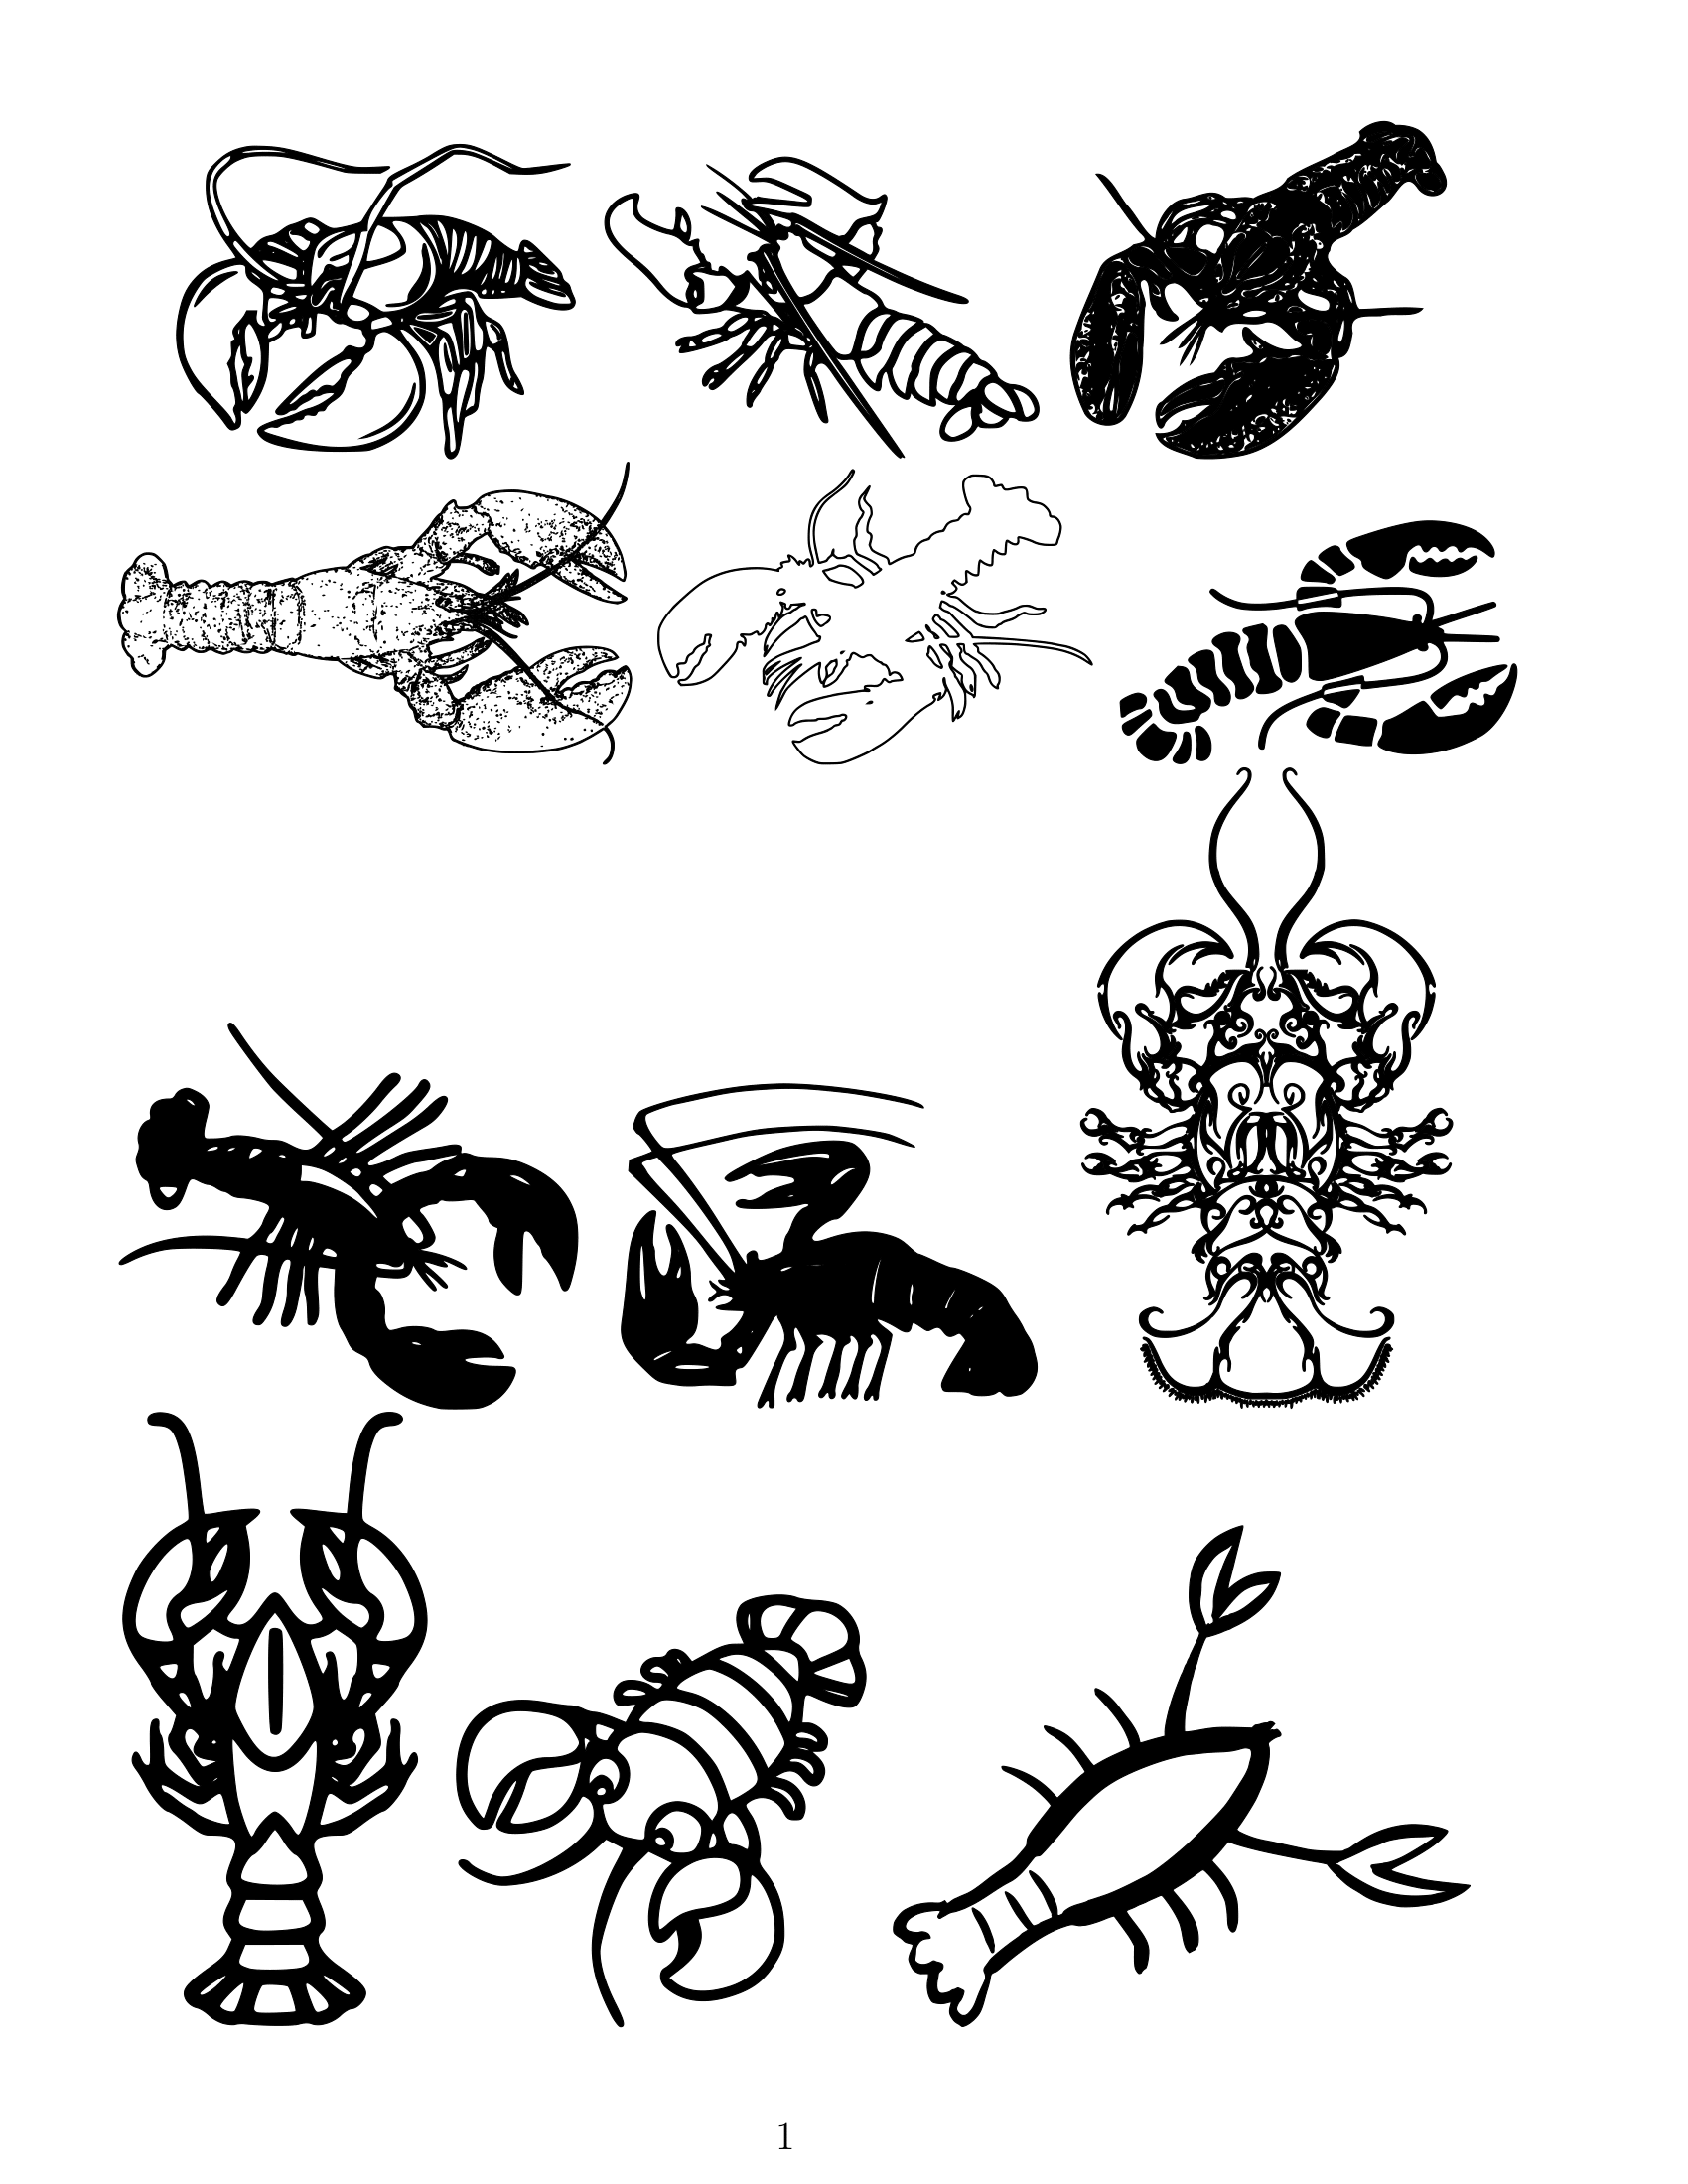
\includegraphics[width=1.2\linewidth]{lobsters_example-1.png}
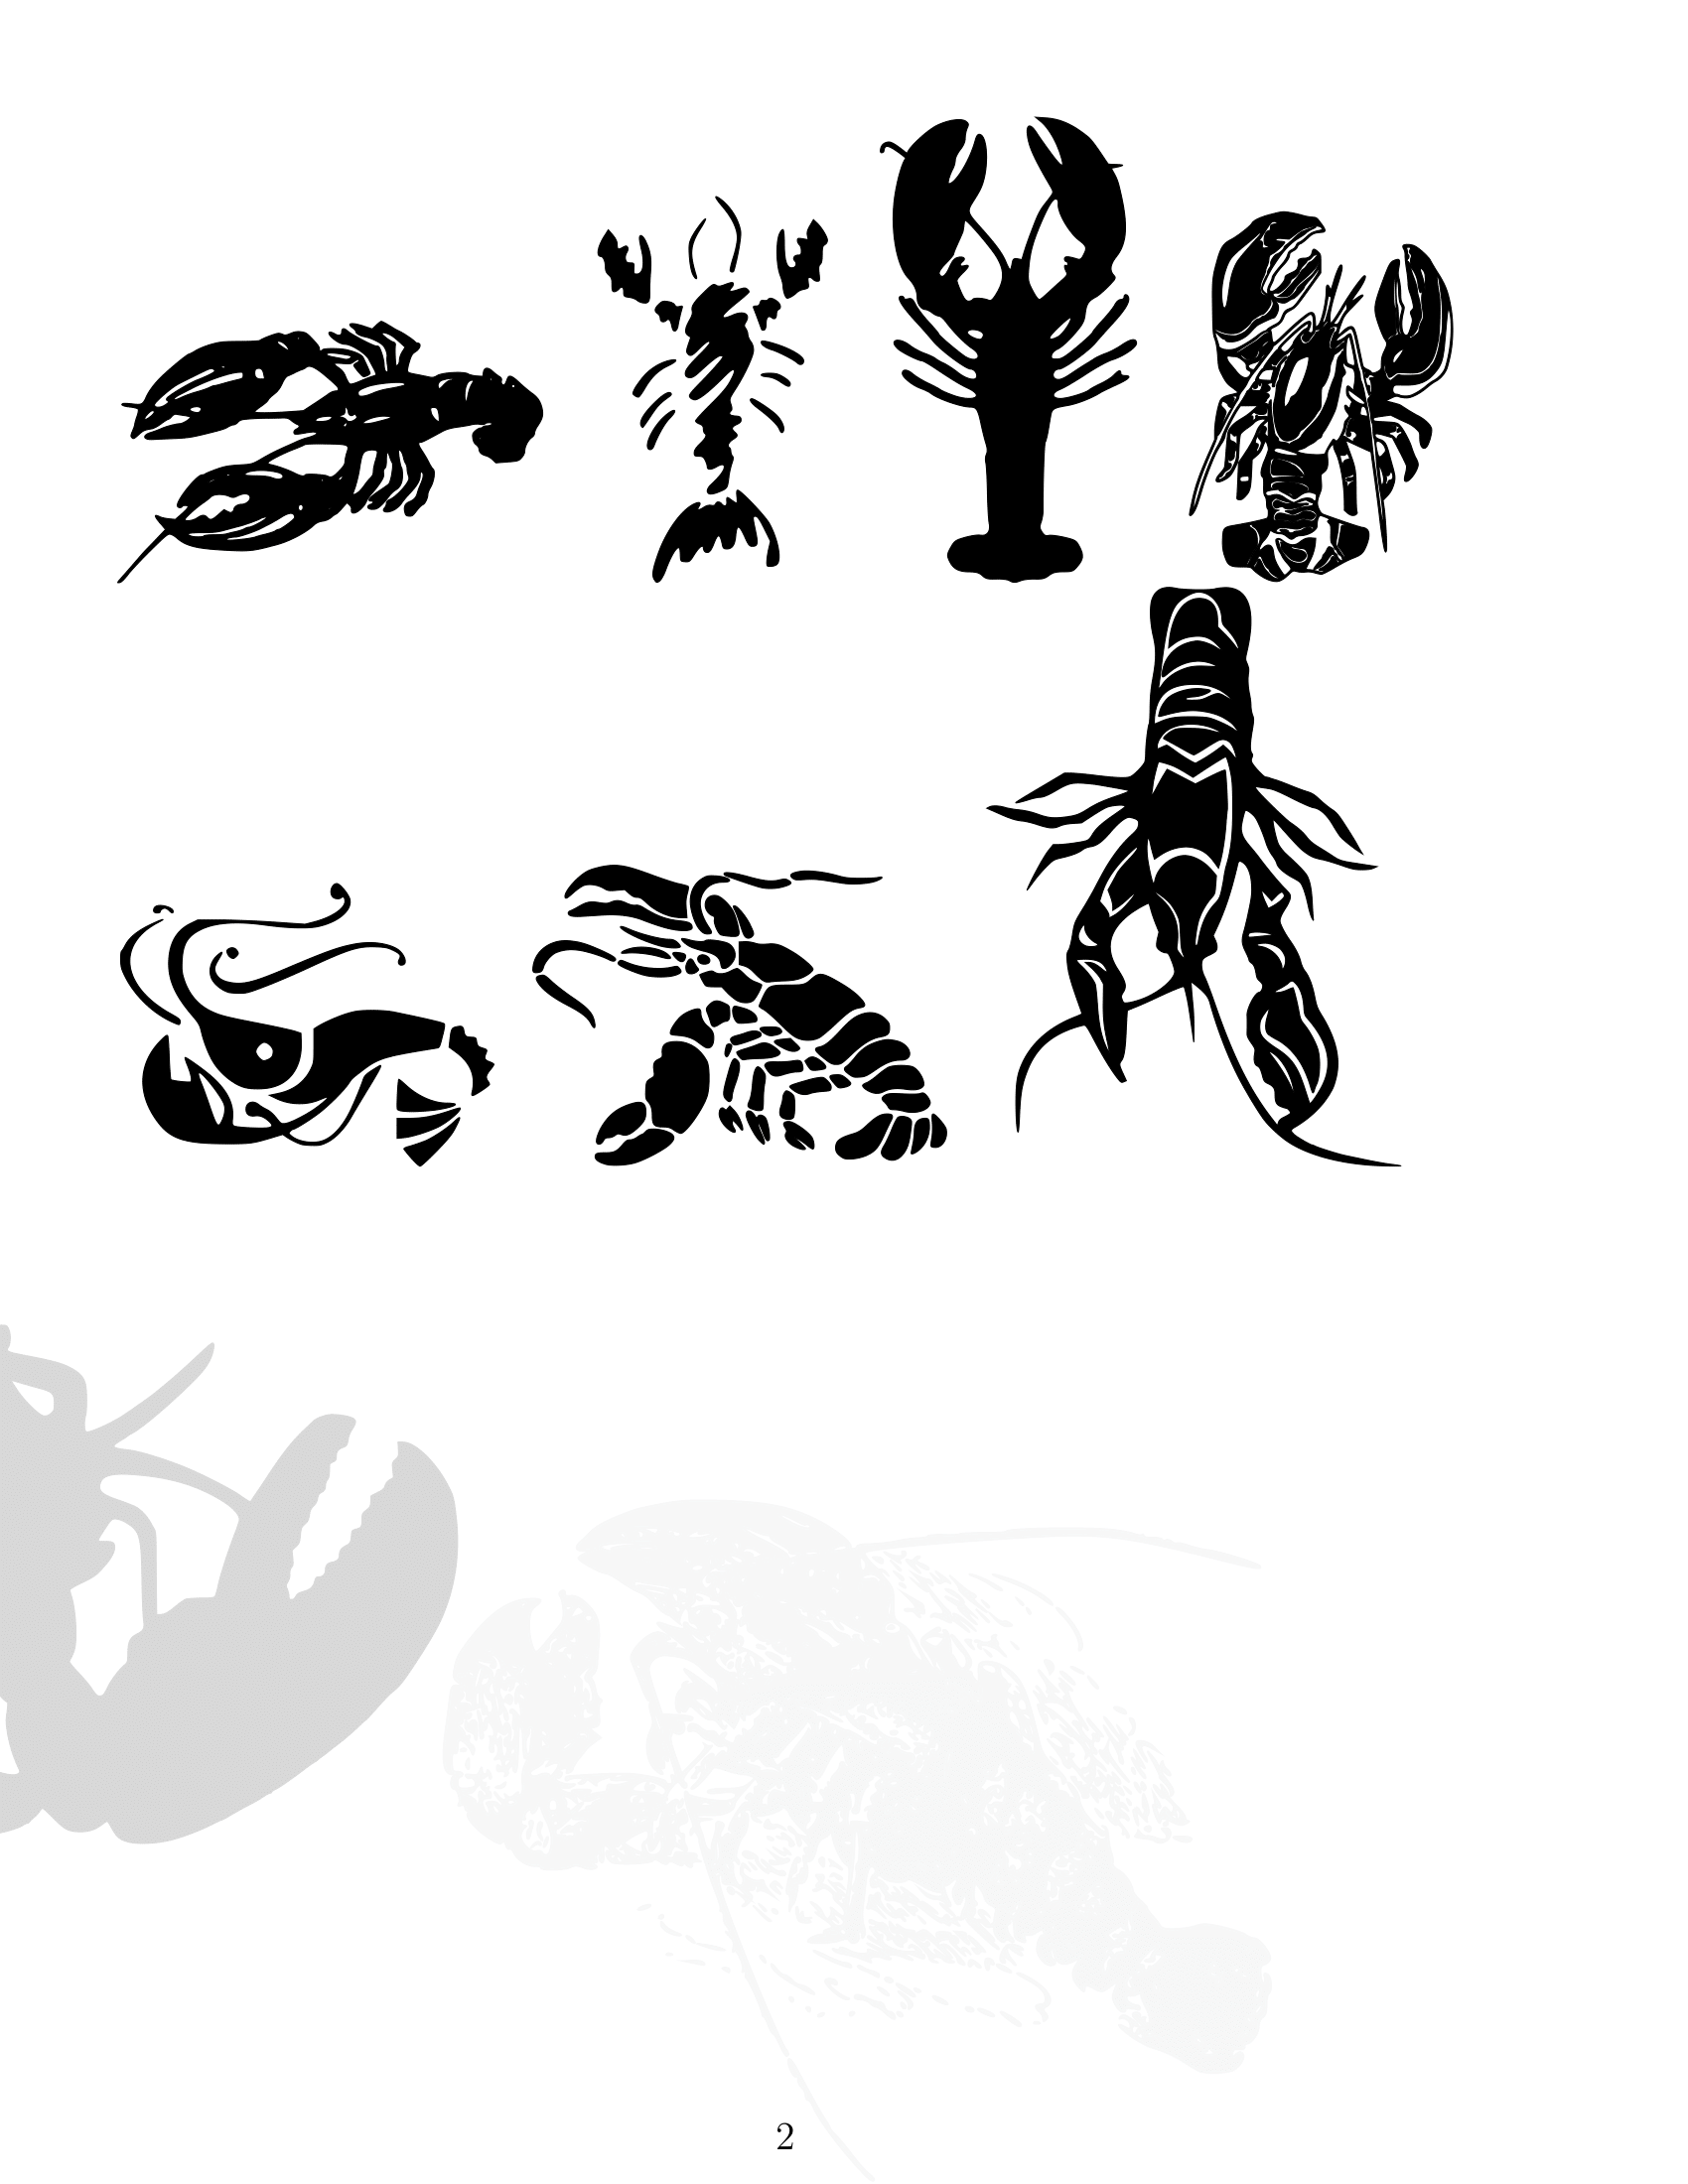
\includegraphics[width=1.2\linewidth]{lobsters_example-2.png}}{\thesubsection}
\end{minipage}
&
\begin{minipage}[m]{0.55\textwidth}
\renewcommand\textminus{\mbox{-}}%<<<<<<<<<<<
\begin{lstlisting}[numberstyle=\zebra{orange!15}{red!15},numbers=left,basicstyle=\ttfamily\scriptsize]
\documentclass[14pt]{extreport}
\usepackage[left=1.5cm,right=3cm,top=1.5cm,
bottom=1.5cm,bindingoffset=0cm]{geometry}
\usepackage{loblib}
 
\begin{document}
\lob{1}     \lob{12}
\lob{2}     \lob{20}
\lob{3}     \lob{21}
\lob{4}     \lob{22}
\lob{5}     \lob{28}
\lob{6}     \lob{32}
\lob{7}     \lob{33}
\lob{8}     \lob{74}
\lob{9}     \lob{76}

\vspace*{2cm}
\hspace*{-2.8cm}
\definecolor{shadow}{rgb}{0.85,0.85,0.85}
\lob[rotate=-90,shadow,xscale=-1.2,yscale=1.2]{77}

\lobwatermark
\end{document}
\end{lstlisting}
LobLib documentation on \href{https://github.com/AnMnv/eBook}{GitHub} in \mybox[black]{LobLib-package} folder.\\ Origins of the package \href{https://github.com/bryce-evans/LobLib}{https://github.com/bryce-evans/LobLib}\\ However, to print lobsters put \mybox[red]{objects} folder and \mybox[red]{loblib.sty} from  the \mybox[black]{LobLib-package} folder into the same directory with your \mybox[brown]{.tex} file.
\end{minipage}
\end{tabular}

%#################### 9.9 ####################
\subsection{\hll{Watermark over \textbf{everything}}}
 
\begin{tabular}{c | c}
\begin{minipage}[m]{0.4\textwidth}
\enum{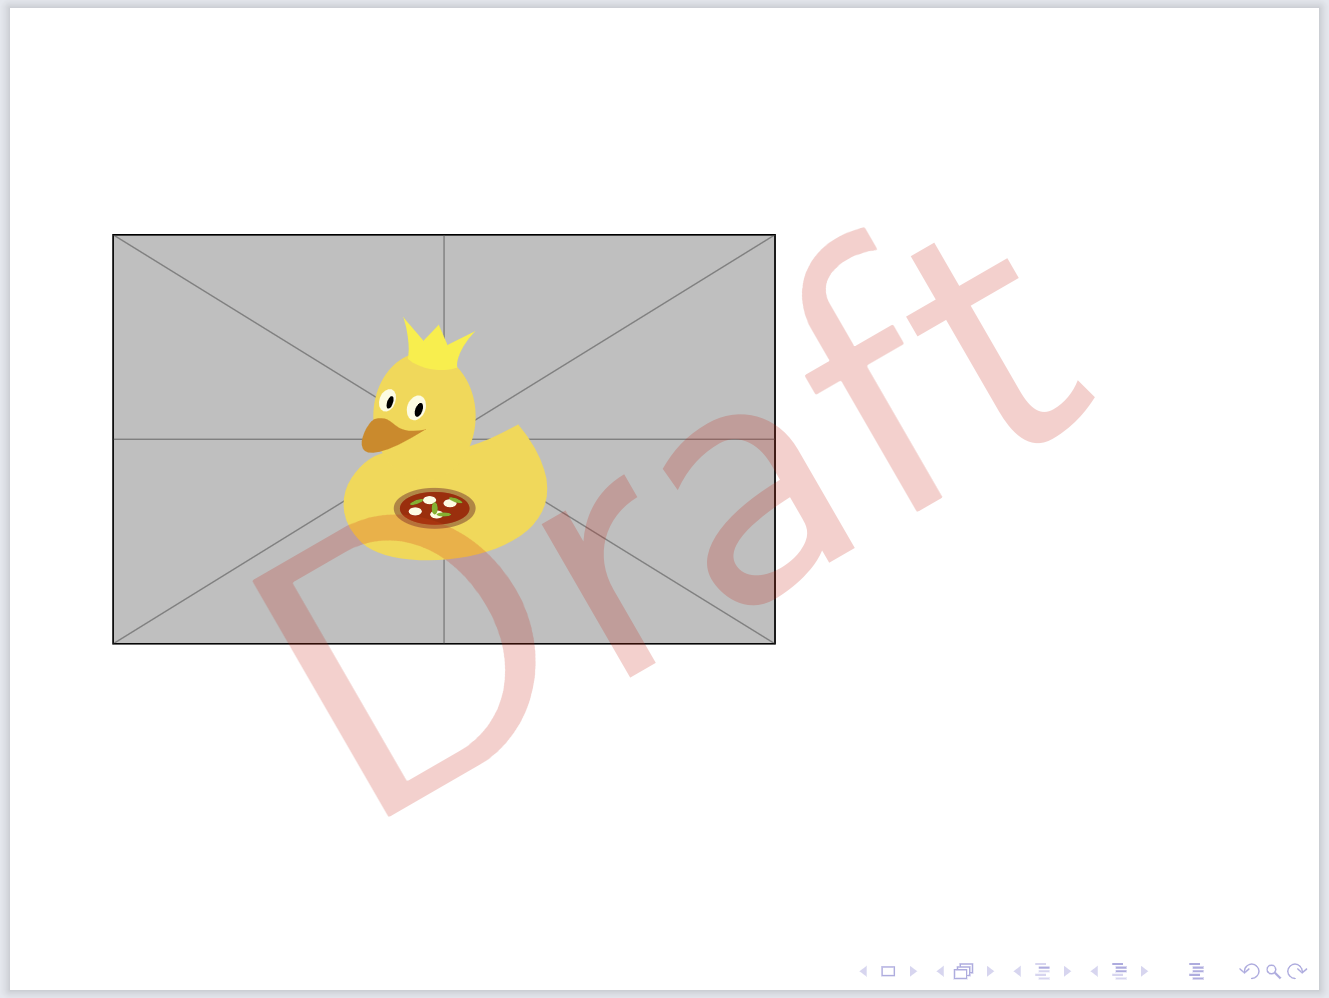
\includegraphics[width=1.\linewidth]{9.9.png}}{}
\end{minipage}
&
\begin{minipage}[m]{0.55\textwidth}
\renewcommand\textminus{\mbox{-}}%<<<<<<<<<<<
\begin{lstlisting}[numberstyle=\zebra{orange!15}{red!15},numbers=left,basicstyle=\ttfamily\scriptsize]
\documentclass{beamer}

\usepackage{tikz}
\AddToHook{shipout/foreground}{
  \begin{tikzpicture}[remember picture,overlay]
    \node[red,rotate=30,scale=10,opacity=0.2] at (current page.center) {Draft}; 
  \end{tikzpicture}}

\begin{document}
\begin{frame}
\includegraphics{example-image-duck}
\end{frame}
\end{document}
\end{lstlisting}
\end{minipage}
\end{tabular}
 
%#################### 9.10 ####################
\subsection{\hll{Simple Emoji by \href{https://github.com/dilippuri/latexemoji}{dilippuri}}}
 
\begin{tabular}{c | c}
\begin{minipage}[m]{0.4\textwidth}
\enum{\href{https://github.com/dilippuri/latexemoji}{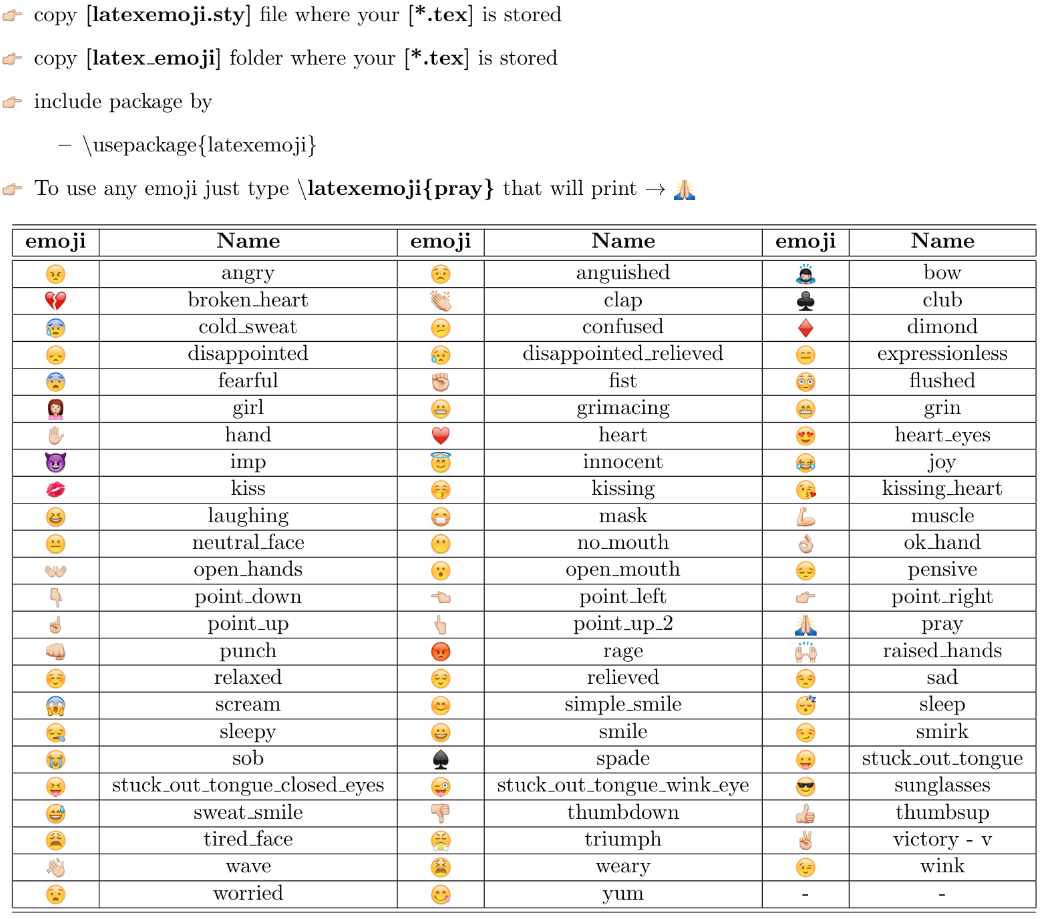
\includegraphics[width=1.\linewidth]{9.10.png}}}{\thesubsection}
\end{minipage}
&
\begin{minipage}[m]{0.55\textwidth}
\renewcommand\textminus{\mbox{-}}%<<<<<<<<<<<
\begin{lstlisting}[numberstyle=\zebra{orange!15}{red!15},numbers=left,basicstyle=\ttfamily\scriptsize]
\documentclass{article} 
\title{This is an example tex file to include emoji in latex}
\author{Dilip Puri}

\begin{document}
\maketitle
Hi, I am (dilippuri) going to include emoji in latex. So I \latexemoji{heart} \LaTeX.\\
I just \latexemoji{stuck_out_tongue_wink_eye}.\\

Good bye! \latexemoji{wave}
\end{document}
\end{lstlisting}
\end{minipage}
\end{tabular}
 
%#################### 9.11####################
\clearpage
...
\vspace{4cm}
...
\subsection{\hll{Confidential mark/ribbon top right of frontpage}}
\begin{tikzpicture}[
  overlay, 
  remember picture,
  legend/.style={|<->|, gray, font = {\ttfamily}},
  confidential/.style={anchor=center, rotate = -45, font={\sffamily\scshape}}
]
  \coordinate (A) at ($ (current page.north east) + (-\stripskip,0) $);
  \coordinate (A') at ($(A) + (-\stripwidth,0) $);

  \coordinate (B) at ($ (current page.north east) + (0,-\stripskip) $);
  \coordinate (B') at ($(B) + (0,-\stripwidth) $);

  \fill [red] (A) -- (A') -- (B') -- (B) -- cycle;

  \coordinate (tempA) at ($(A)!.5!(A')$);
  \coordinate (tempB) at ($(B)!.5!(B')$);

  \node [confidential](text) at ($(tempA)!.5!(tempB)$) {\Huge Confidential};
\end{tikzpicture}
 
\begin{tabular}{c | c}
\begin{minipage}[m]{0.4\textwidth}
 Look at the top right of the page
\end{minipage}
&
\begin{minipage}[m]{0.55\textwidth}
\renewcommand\textminus{\mbox{-}}%<<<<<<<<<<<
\begin{lstlisting}[numberstyle=\zebra{orange!15}{red!15},numbers=left,basicstyle=\ttfamily\scriptsize]
\documentclass{article} 
\documentclass{scrbook}
\usepackage{lmodern}
\usepackage{tikz}
\usetikzlibrary{calc}
\newcommand{\stripskip}{5}
\newcommand{\stripwidth}{3}

\begin{document}
    \begin{tikzpicture}[
        overlay, 
        remember picture,
        legend/.style={|<->|, gray, font = {\ttfamily}},
        confidential/.style={anchor=center, rotate = -45, font={\sffamily\scshape}}
    ]
        \coordinate (A) at ($ (current page.north east) + (-\stripskip,0) $);
        \coordinate (A') at ($(A) + (-\stripwidth,0) $);

        \coordinate (B) at ($ (current page.north east) + (0,-\stripskip) $);
        \coordinate (B') at ($(B) + (0,-\stripwidth) $);

        \fill [red] (A) -- (A') -- (B') -- (B) -- cycle;

        \coordinate (tempA) at ($(A)!.5!(A')$);
        \coordinate (tempB) at ($(B)!.5!(B')$);

        \node [confidential](text) at ($(tempA)!.5!(tempB)$) {\Huge Confidential};
    \end{tikzpicture}
    \centering \Huge qqqqqqqqq
\end{document}
\end{lstlisting}
\end{minipage}
\end{tabular}
 
 
%#################### 9.12 ####################
\subsection{\hll{Text in different shapes}}
 
\begin{tabular}{c | c}
\begin{minipage}[m]{0.4\textwidth}
\enum{\shapepar{\heartshape}{\small Happy families are all alike; every unhappy family is unhappy in its own way. Happy families are all alike; every unhappy family is unhappy in its own way.}}{\thesubsection}


Available shapes: hexagonshape, heartshape,diamondshape, nutshape, starshape


\end{minipage}
&
\begin{minipage}[m]{0.55\textwidth}
\renewcommand\textminus{\mbox{-}}%<<<<<<<<<<<
\begin{lstlisting}[numberstyle=\zebra{orange!15}{red!15},numbers=left,basicstyle=\ttfamily\scriptsize]
\documentclass{article}
\usepackage{blindtext}
\usepackage{shapepar}

\begin{document}
\shapepar{\heartshape}{\blindtext[1]}
\end{document}
\end{lstlisting}
\end{minipage}
\end{tabular}
 
%#################### 9.13 #################### https://tex.stackexchange.com/questions/712250/drawing-3d-dice

\subsection{\hll{Drawing 3D dice}}
 
\begin{tabular}{c | c}
\begin{minipage}[m]{0.4\textwidth}
\enum{\href{https://tex.stackexchange.com/questions/712250/drawing-3d-dice}{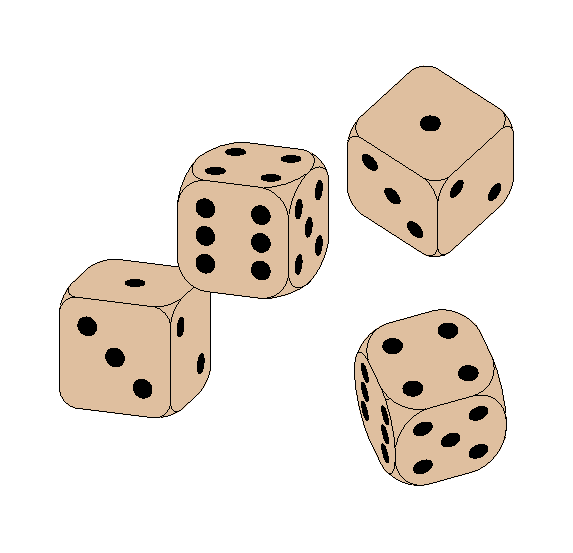
\includegraphics[width=1.\linewidth]{9.13.pdf}}}{\thesubsection}
\end{minipage}
&
\begin{minipage}[m]{0.55\textwidth}
\renewcommand\textminus{\mbox{-}}%<<<<<<<<<<<
\begin{lstlisting}[numberstyle=\zebra{orange!15}{red!15},numbers=left,basicstyle=\ttfamily\scriptsize]
  \documentclass[tikz, border=1cm]{standalone}
  \usepackage{tikz-3dplot}
  \begin{document}
  \newcommand{\dicenum}[1]{%
  \pgfmathparse{#1==2 || #1==4 || #1==5 || #1==6}\ifnum\pgfmathresult>0\relax%
  \fill[black] (0.5,0.5) circle[radius=1/6];    % top left
  \fill[black] (-0.5,-0.5) circle[radius=1/6];\fi % bottom right
  \pgfmathparse{#1==3 || #1==4 || #1==5 || #1==6}\ifnum\pgfmathresult>0\relax%
  \fill[black] (-0.5,0.5) circle[radius=1/6];    % top right
  \fill[black] (0.5,-0.5) circle[radius=1/6];\fi % bottom left
  \pgfmathparse{#1==1 || #1==3 || #1==5}\ifnum\pgfmathresult>0\relax%
  \fill[black] (0,0) circle[radius=1/6]; \fi % center
  \ifnum#1=6\relax%
  \fill[black] (0.5,0) circle[radius=1/6];     % middle left
  \fill[black] (-0.5,0) circle[radius=1/6];\fi % middle right
  }
  \newcounter{currnum}
  \setcounter{currnum}{1}
  \begin{tikzpicture}
  \newcommand{\dice}[5]{
  \tdplotsetmaincoords{#3}{#4}
  \begin{scope}[shift={(#1,#2)}, tdplot_main_coords, rounded corners=#5, fill=brown!50!white]
  \begin{scope}[canvas is xy plane at z=-1]
  \filldraw (-1,-1) rectangle (1,1);
  \end{scope}
  \begin{scope}[canvas is xz plane at y=-1]
  \filldraw (-1,-1) rectangle (1,1);
  \end{scope}
  \begin{scope}[canvas is yz plane at x=-1]
  \filldraw (-1,-1) rectangle (1,1);
  \end{scope}
  \begin{scope}[canvas is xy plane at z=1]
  \filldraw (-1,-1) rectangle (1,1);
  \dicenum{\value{currnum}}
  \stepcounter{currnum}
  \ifnum\value{currnum}>6\relax\setcounter{currnum}{1}\fi
  \end{scope}
  \begin{scope}[canvas is xz plane at y=1]
  \filldraw (-1,-1) rectangle (1,1);
  \dicenum{\value{currnum}}
  \stepcounter{currnum}
  \ifnum\value{currnum}>6\relax\setcounter{currnum}{1}\fi
  \end{scope}
  \begin{scope}[canvas is yz plane at x=1]
  \filldraw (-1,-1) rectangle (1,1);
  \dicenum{\value{currnum}}
  \stepcounter{currnum}
  \ifnum\value{currnum}>6\relax\setcounter{currnum}{1}\fi
  \end{scope}
  \end{scope}
  }
  \dice{0}{0}{70}{110}{0.3cm};
  \dice{2}{2}{70}{110}{0.5cm};
  \dice{5}{3}{40}{130}{0.3cm};
  \dice{5}{-1}{40}{160}{0.6cm};
  \end{tikzpicture}
  \end{document}
\end{lstlisting}
\end{minipage}
\end{tabular}
 

%#################### 9.14 #################### https://ctan.org/pkg/tikzlings
 
\subsection{\hll{Animals}}
 
\begin{tabular}{c | c}
\begin{minipage}[m]{0.4\textwidth}
  \begin{tikzpicture}
  \bat[
    signpost={AnMnV},
    signcolour= brown!50!black,
    signback=green!40!black
    ]
  \end{tikzpicture}
  \begin{tikzpicture}
  \marmot
  \end{tikzpicture}
  \begin{tikzpicture}
  \anteater
  \end{tikzpicture}
  \begin{tikzpicture}
  \wolf 
  \end{tikzpicture}
  \begin{tikzpicture}
  \bear
  \end{tikzpicture}
  \begin{tikzpicture}
  \bee
  \end{tikzpicture}
  \begin{tikzpicture}
  \bug
  \end{tikzpicture}
  \begin{tikzpicture}
  \cat
  \end{tikzpicture}
  \begin{tikzpicture}
  \squirrel
  \end{tikzpicture}
  \begin{tikzpicture}
  \snowman
  \end{tikzpicture}
  \begin{tikzpicture}
  \sloth
  \end{tikzpicture}
  \begin{tikzpicture}
  \sheep
  \end{tikzpicture}
  \begin{tikzpicture}
  \pig
  \end{tikzpicture}
  \begin{tikzpicture}
  \rhino
  \end{tikzpicture}
  \begin{tikzpicture}
  \penguin
  \end{tikzpicture}
  \begin{tikzpicture}
  \panda
  \end{tikzpicture}
  \begin{tikzpicture}
  \owl
  \end{tikzpicture}
  \begin{tikzpicture}
  \chicken
  \end{tikzpicture}
  \begin{tikzpicture}
  \mouse
  \end{tikzpicture}
  \begin{tikzpicture}
  \coati
  \end{tikzpicture}
  \begin{tikzpicture}
  \elephant
  \end{tikzpicture}
  \begin{tikzpicture}
  \hippo
  \end{tikzpicture}
  \begin{tikzpicture}
  \koala
  \end{tikzpicture}
\end{minipage}
&
\begin{minipage}[m]{0.55\textwidth}
\renewcommand\textminus{\mbox{-}}%<<<<<<<<<<<
\begin{lstlisting}[numberstyle=\zebra{orange!15}{red!15},numbers=left,basicstyle=\ttfamily\scriptsize]
\documentclass{standalone}
\usepackage{tikzlings}
\begin{document}

\begin{tikzpicture}
\marmot
\end{tikzpicture}	

\end{document}
\end{lstlisting}
\begin{tcolorbox}[colback=red!5,colframe=red!75!black,
title=Evailable creacures: ]
\begin{multicols}{2}%change to have more columns
  \begin{enumerate}
    \item anteater
    \item bat
    \item bear
    \item bee
    \item bug
    \item cat
    \item chicken
    \item coati
    \item hippo
    \item elephant
    \item koala
    \item marmot
    \item mole
    \item mouse
    \item owl
    \item panda
    \item penguin
    \item pig
    \item rhino
    \item sheep
    \item sloth
    \item snowman
    \item squirrel
    \item wolf
  \end{enumerate}
  \end{multicols}
\href{https://ctan.org/pkg/tikzlings}{https://ctan.org/pkg/tikzlings}
\end{tcolorbox}
\end{minipage}
\end{tabular}
 
%#################### 9.15 #################### 

\subsection{\hll{Skill icons \photosymbol{Git} \photosymbol{LaTeX-Dark} \photosymbol{Linux-Light} \photosymbol{Github-Dark} \photosymbol{VSCode-Light}}}

\begin{tabular}{c | c}
\begin{minipage}[m]{0.4\textwidth}
\photosymbol[3]{Ableton-Dark}
\photosymbol[3]{Ableton-Light}
\photosymbol[3]{ActivityPub-Dark}
\photosymbol[3]{ActivityPub-Light}
\photosymbol[3]{Actix-Dark}
\photosymbol[3]{Actix-Light}
\photosymbol[3]{Adonis}
\photosymbol[3]{AfterEffects}
\photosymbol[3]{AiScript-Dark}
\photosymbol[3]{AiScript-Light}
\photosymbol[3]{AlpineJS-Dark}
\photosymbol[3]{AlpineJS-Light}
\photosymbol[3]{Anaconda-Dark}
\photosymbol[3]{Anaconda-Light}
\photosymbol[3]{AndroidStudio-Dark}
\photosymbol[3]{AndroidStudio-Light}
\photosymbol[3]{Angular-Dark}
\photosymbol[3]{Angular-Light}
\photosymbol[3]{Ansible}
\photosymbol[3]{Apollo}
\photosymbol[3]{Apple-Dark}
\photosymbol[3]{Apple-Light}
\photosymbol[3]{Appwrite}
\photosymbol[3]{Arch-Dark}
\photosymbol[3]{Arch-Light}
\photosymbol[3]{Arduino}
\photosymbol[3]{Astro}
\photosymbol[3]{Atom}
\photosymbol[3]{Audition}
\photosymbol[3]{Autocad-Light}
\photosymbol[3]{AWS-Dark}
\photosymbol[3]{AWS-Light}
\photosymbol[3]{Azul}
\photosymbol[3]{Azure-Dark}
\photosymbol[3]{Azure-Light}
\photosymbol[3]{Babel}
\photosymbol[3]{Bash-Dark}
\photosymbol[3]{Bash-Light}
\photosymbol[3]{Bevy-Dark}
\photosymbol[3]{Bevy-Light}
\photosymbol[3]{BitBucket-Dark}
\photosymbol[3]{BitBucket-Light}
\photosymbol[3]{Blender-Dark}
\photosymbol[3]{Blender-Light}
\photosymbol[3]{Bootstrap}
\photosymbol[3]{BSD-Dark}
\photosymbol[3]{BSD-Light}
\photosymbol[3]{Bun-Dark}
\photosymbol[3]{Bun-Light}
\photosymbol[3]{C}
\photosymbol[3]{Cassandra-Dark}
\photosymbol[3]{Cassandra-Light}
\photosymbol[3]{CLion-Dark}
\photosymbol[3]{CLion-Light}
\photosymbol[3]{Clojure-Dark}
\photosymbol[3]{Clojure-Light}
\photosymbol[3]{Cloudflare-Dark}
\photosymbol[3]{Cloudflare-Light}
\photosymbol[3]{CMake-Dark}
\photosymbol[3]{CMake-Light}
\photosymbol[3]{CodePen-Dark}
\photosymbol[3]{CodePen-Light}
\photosymbol[3]{CoffeeScript-Dark}
\photosymbol[3]{CoffeeScript-Light}
\photosymbol[3]{CPP}
\photosymbol[3]{Crystal-Dark}
\photosymbol[3]{Crystal-Light}
\photosymbol[3]{CS}
\photosymbol[3]{CSS}
\photosymbol[3]{Cypress-Dark}
\photosymbol[3]{Cypress-Light}
\photosymbol[3]{D3-Dark}
\photosymbol[3]{D3-Light}
\photosymbol[3]{Dart-Dark}
\photosymbol[3]{Dart-Light}
\photosymbol[3]{Debian-Dark}
\photosymbol[3]{Debian-Light}
\photosymbol[3]{DENO-Dark}
\photosymbol[3]{DENO-Light}
\photosymbol[3]{DevTo-Dark}
\photosymbol[3]{DevTo-Light}
\photosymbol[3]{Discord}
\photosymbol[3]{DiscordBots}
\photosymbol[3]{DiscordJS-Dark}
\photosymbol[3]{DiscordJS-Light}
\photosymbol[3]{Django}
\photosymbol[3]{Docker}
\photosymbol[3]{DotNet}
\photosymbol[3]{DynamoDB-Dark}
\photosymbol[3]{Eclipse-Dark}
\photosymbol[3]{Eclipse-Light}
\photosymbol[3]{Elasticsearch-Dark}
\photosymbol[3]{Elasticsearch-Light}
\photosymbol[3]{Electron}
\photosymbol[3]{Elixir-Dark}
\photosymbol[3]{Elixir-Light}
\photosymbol[3]{Elysia-Dark}
\photosymbol[3]{Emacs}
\photosymbol[3]{Ember}
\photosymbol[3]{Emotion-Dark}
\photosymbol[3]{Emotion-Light}
\photosymbol[3]{ExpressJS-Dark}
\photosymbol[3]{ExpressJS-Light}
\photosymbol[3]{FastAPI}
\photosymbol[3]{Fediverse-Dark}
\photosymbol[3]{Fediverse-Light}
\photosymbol[3]{Figma-Dark}
\photosymbol[3]{Figma-Light}
\photosymbol[3]{Firebase-Dark}
\photosymbol[3]{Firebase-Light}
\photosymbol[3]{Flask-Dark}
\photosymbol[3]{Flask-Light}
\photosymbol[3]{Flutter-Dark}
\photosymbol[3]{Forth}
\photosymbol[3]{Fortran}
\photosymbol[3]{GameMakerStudio}
\photosymbol[3]{Gatsby}
\photosymbol[3]{GCP-Dark}
\photosymbol[3]{Gherkin-Dark}
\photosymbol[3]{Git}
\photosymbol[3]{Github-Dark}
\photosymbol[3]{GithubActions-Light}
\photosymbol[3]{GitLab-Light}
\photosymbol[3]{Gmail-Dark}
\photosymbol[3]{Godot-Dark}
\photosymbol[3]{GoLang}\\[0.5cm]

AND MUCH MORE !
\end{minipage}
&
\begin{minipage}[m]{0.55\textwidth}
\renewcommand\textminus{\mbox{-}}%<<<<<<<<<<<
\begin{lstlisting}[numberstyle=\zebra{orange!15}{red!15},numbers=left,basicstyle=\ttfamily\normalsize]
\documentclass[11pt]{report}
\usepackage{skillicons}
\begin{document}
\begin{itemize}
\item[] \photosymbol{JavaScript} I'm proficient in JavaScript.
\item[] \photosymbol{Python-Dark} Python is one of my core skills.
\item[] \photosymbol{React-Light} I have experience working with React.
\item[] \photosymbol{Java-Dark} Java is one of my strong suits.
\item[] \photosymbol{NodeJS-Light} I'm proficient in Node.js development.
\item[] \photosymbol{Git} I'm adept at using Git for version control.
\item[] \photosymbol{MySQL-Dark} SQL is one of the databases languages.
\item[] \photosymbol{Rust} Rust is a language I've been learning and enjoying lately.
\end{itemize}
\end{document}
\end{lstlisting}

SEE FULL INSTRUCTION OF USING  \xmyboxg{skillicons} package here: 
\href{https://github.com/AnMnv/latex-skill-icons}{https://github.com/AnMnv/latex-skill-icons}
\end{minipage}
\end{tabular}